\RequirePackage{ifpdf}
\ifpdf
	\documentclass[11pt,oneside,a4paper,pdftex]{article}   %two-page printing
\else
	\documentclass[11pt,twoside,a4paper,dvips]{article}   %two-page printing
\fi

%\documentclass[a4paper, 12pt]{article}
\addtolength{\hoffset}{-1.9cm}
\addtolength{\voffset}{-1.9cm}
\addtolength{\textwidth}{+3.8cm}
\addtolength{\textheight}{+3.8cm}
\usepackage[latin1,utf8]{inputenc}
\usepackage[czech]{babel}
\usepackage{icomma} % ceska desetinna carka
\usepackage{csquotes}
\usepackage{listings}
\usepackage{amsmath}
\usepackage{amsthm}
\usepackage{amsfonts}
\usepackage{mathrsfs}
%\usepackage[T1]{fontenc}
\ifpdf
	\usepackage[pdftex]{graphicx} % dvips or pdftex
\else
	\usepackage[dvips]{graphicx} % dvips or pdftex
\fi
\usepackage[center]{subfigure}
\usepackage{amsfonts}
\usepackage[dvips]{color}               %for using colors
%\usepackage{showframe}                 %zobrazuje okraje stranky
\usepackage[justification=justified,hang]{caption}
\usepackage{textpos}
\usepackage{url}
%\usepackage{fancybox}
\usepackage{verbatim}
\usepackage{fj}
\ifpdf
	\usepackage[pdftex,unicode,colorlinks]{hyperref}
\else
	\usepackage[unicode]{hyperref}
\fi


%FIXME: odlišit font, aby části kódu byly odlišitelné od okolního textu
\lstset{ %
language=Matlab,           % choose the language of the code
basicstyle=\ttfamily,   % the size of the fonts that are used for the code
numbers=none,             % where to put the line-numbers (none, left, ..)
numberstyle=\scriptsize,  % size of the fonts used for the line-numbers
stepnumber=1,             % step between two line-nums. If "1" each line nmbrd
numbersep=10pt,            % how far the line-numbers are from the code
%backgroundcolor=\color{white},
	% choose the background color. You must add \usepackage{color}
showspaces=false,         % show spaces adding particular underscores
showstringspaces=false,   % underline spaces within strings
showtabs=false,           % show tabs within strings
frame=none,	          % adds a frame around the code (single, none, ...)
tabsize=2,	          % sets default tabsize to 2 spaces
captionpos=b,             % sets the caption-position to bottom
breaklines=false,          % sets automatic line breaking
breakatwhitespace=true,   % sets if automatic breaks should only happen at \s
%escapeinside={\%*}{*)}   % if you want to add a comment within your code
}

\title{1. Zpráva pro předmět 3D Počítačové vidění -- A4M33TDV}
\date{29. 11. 2011}
\author{Filip Jareš, jaresfil@fel.cvut.cz}

\begin{document}

\maketitle

\section{Úvod}

Tato zpráva popisuje semestrální práci pro předmět 3D počítačové vidění, jejímž cílem je na základě
dvanácti fotografií vybraného objektu (portálu/dveří) zrekonstruovat nasnímanou scénu a vytvořit
trojrozměrný digitální model této scény.

Práce ještě není dokončená, proto v této verzi zpráva popisuje pouze dosud hotovou část řešení:
výběr scény, zvolenou konfiguraci kamer, nástroj použitý pro odstranění radiálního zkreslení
a~metodu kalibrace kamery. Nakonec potom hledání řídkých korespondencí mezi obrazy a~odhad
epipolární geometrie mezi dvojicemi snímků.

\section{Řešení}

\subsection{Struktura řešení}

Použité řešení úlohy rekonstrukce 3D scény z několika fotografií lze rozdělit na tři hlavní fáze:
(1) zachycení scény a přípravu snímků pro pozdější zpracování; (2) rekonstrukci řídkého mraku
prostorových bodů z~těchto snímků a (3) rekonstrukci hustého mraku bodů s použitím stereo párování,
které poskytne husté korespondence mezi dvojicemi obrazů se známou epipolární geometrií.
Tato první verze zprávy popisuje pouze fázi první a částečně fázi druhou.

Důležitým krokem fáze (1) je odstranění radiálního zkreslení. Hlavními částmi fáze (2) je nalezení
řídkých korespondencí mezi obrazy a použití těchto korespondencí k odhadu epipolární geometrie
dvojic snímků a tedy odhadu relativních rotací a translací dvojic kamer. Následuje \uv{slepování}
takových dvojic kamer, tedy jejich umístění do společného souřadného systému.

V následující části jsou jednotlivé kroky prvních dvou fází (kromě \uv{slučování} kamer) popsány
podrobněji.

\subsection{Popis řešení}

\paragraph{Výběr scény}
Jako objekt pro rekonstrukci byly vybrány domovní dveře domu v pražské Jeseniově ulici. Byly
vyfotografovány z dvanácti míst tak, jak je to přibližně znázorněno na \figref{fig:usporadaniKamer}.
Kolmá vzdálenost od dveří byla u všech kamer přibližně stejná (zhruba 4\,m) a dveře byly ze čtyř
míst vyfotografovány vždy ze tří rúzných výškových úrovní (zhruba z výšky 30\,cm, 130\,cm a
200\,cm).
	\begin{figure}[h]
		\centering
		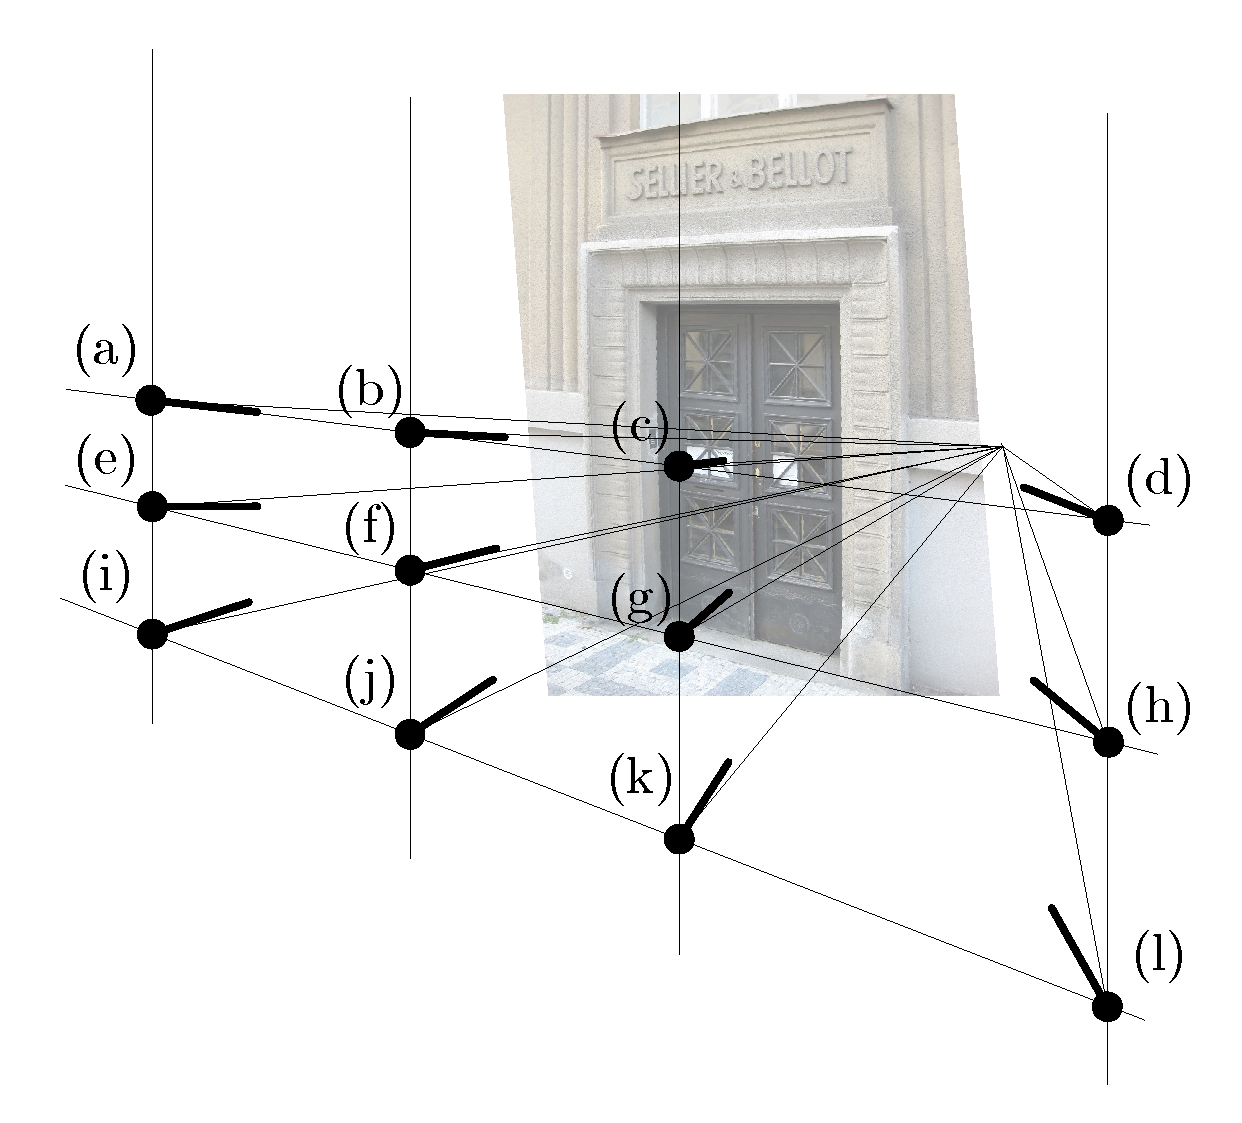
\includegraphics[width=8cm]{pictures/usporadani_kamer.pdf}
		\caption{Schéma uspořádání kamer při snímání scény}
		\label{fig:usporadaniKamer}
	\end{figure}
Fotografie s rozlišením $3264\times2448$ pixelů byly pořízeny fotoaparátem Canon Ixus 80
IS na nejkratší ohniskovou vzdálenost. Zachyceny jsou na \figref{fig:fotografie}.
	\begin{figure}[htbp]
		% dummy content, to make the rendering faster while under construction
			\centering
			\subfigure[] {
				\fbox{\begin{minipage}{3cm}\hfill\vspace{4cm}\end{minipage}}
				\label{fig:firstInputImage}
			}
			\subfigure[] {
				\fbox{\begin{minipage}{3cm}\hfill\vspace{4cm}\end{minipage}}
			}
			\subfigure[] {
				\fbox{\begin{minipage}{3cm}\hfill\vspace{4cm}\end{minipage}}
			}
			\subfigure[] {
				\fbox{\begin{minipage}{3cm}\hfill\vspace{4cm}\end{minipage}}
			}
			\\
			\subfigure[] {
				\fbox{\begin{minipage}{3cm}\hfill\vspace{4cm}\end{minipage}}
			}
			\subfigure[] {
				\fbox{\begin{minipage}{3cm}\hfill\vspace{4cm}\end{minipage}}
				\label{fig:i0}
			}
			\subfigure[] {
				\fbox{\begin{minipage}{3cm}\hfill\vspace{4cm}\end{minipage}}
				\label{fig:i1}
			}
			\subfigure[] {
				\fbox{\begin{minipage}{3cm}\hfill\vspace{4cm}\end{minipage}}
			}
			\\
			\subfigure[] {
				\fbox{\begin{minipage}{3cm}\hfill\vspace{4cm}\end{minipage}}
			}
			\subfigure[] {
				\fbox{\begin{minipage}{3cm}\hfill\vspace{4cm}\end{minipage}}
			}
			\subfigure[] {
				\fbox{\begin{minipage}{3cm}\hfill\vspace{4cm}\end{minipage}}
			}
			\subfigure[] {
				\fbox{\begin{minipage}{3cm}\hfill\vspace{4cm}\end{minipage}}
			}
		% Real pictures:
			% \centering
			% \subfigure[] {
			% 	\fbox{\includegraphics[width=4cm,angle=-90]{pictures/IMG_5959.JPG}}
			%	\label{fig:firstInputImage}
			% }
			% \subfigure[] {
			% 	\fbox{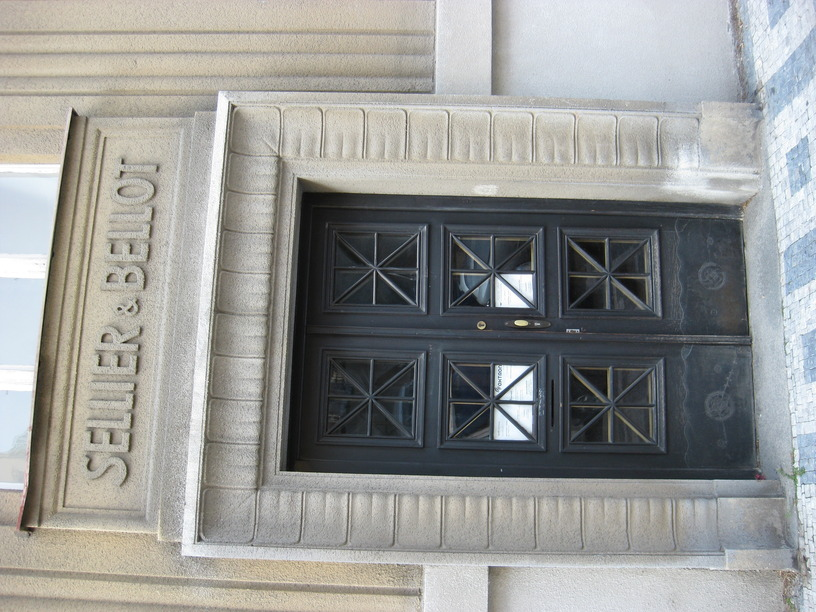
\includegraphics[width=4cm,angle=-90]{pictures/IMG_5955.JPG}}
			% }
			% \subfigure[] {
			% 	\fbox{\includegraphics[width=4cm,angle=-90]{pictures/IMG_5962.JPG}}
			% }
			% \subfigure[] {
			% 	\fbox{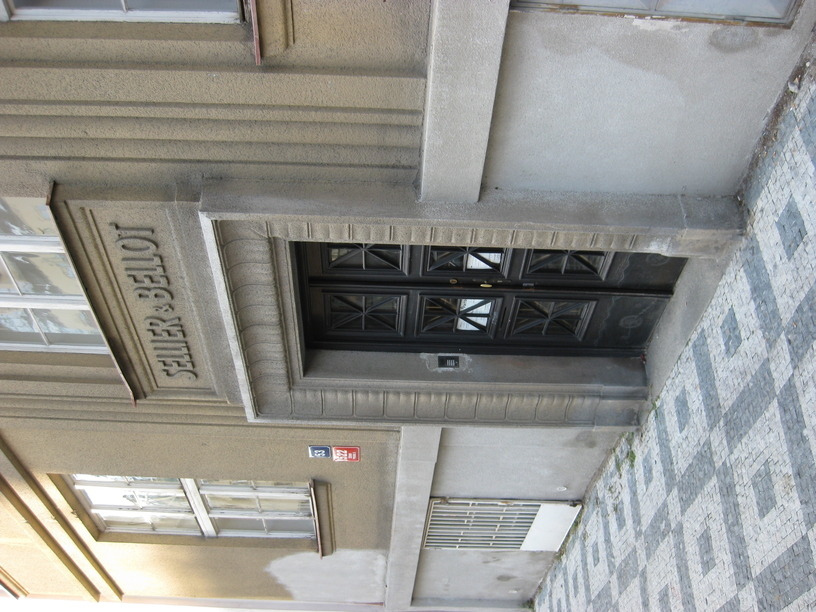
\includegraphics[width=4cm,angle=-90]{pictures/IMG_5965.JPG}}
			% }
			% \\
			% \subfigure[] {
			% 	\fbox{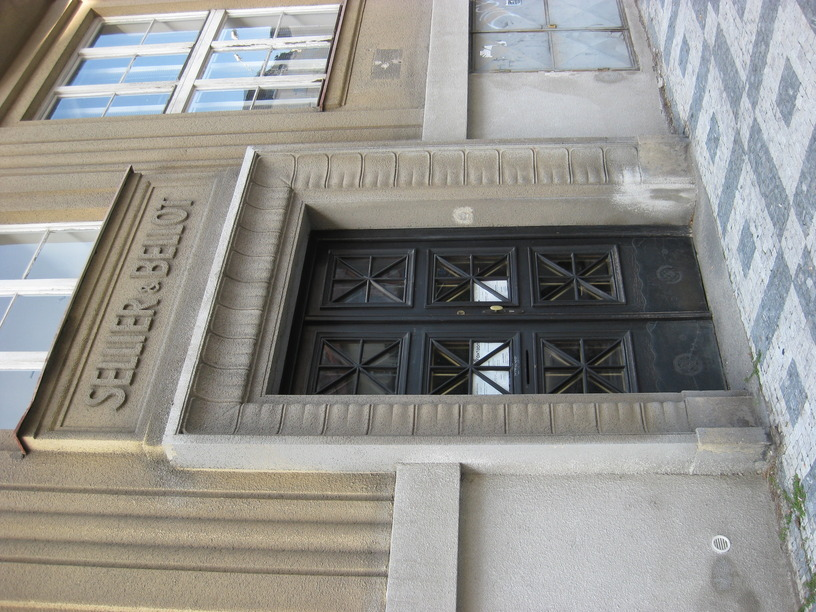
\includegraphics[width=4cm,angle=-90]{pictures/IMG_5957.JPG}}
			% }
			% \subfigure[] {
			% 	\fbox{\includegraphics[width=4cm,angle=-90]{pictures/IMG_5954.JPG}}
			%	\label{fig:i0}
			% }
			% \subfigure[] {
			% 	\fbox{\includegraphics[width=4cm,angle=-90]{pictures/IMG_5961.JPG}}
			%	\label{fig:i1}
			% }
			% \subfigure[] {
			% 	\fbox{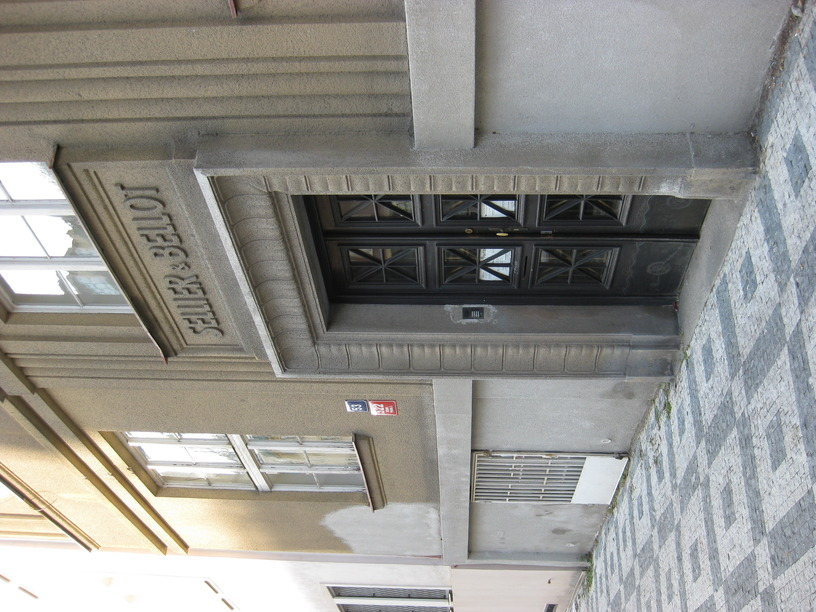
\includegraphics[width=4cm,angle=-90]{pictures/IMG_5964.JPG}}
			% }
			% \\
			% \subfigure[] {
			% 	\fbox{\includegraphics[width=4cm,angle=-90]{pictures/IMG_5956.JPG}}
			% }
			% \subfigure[] {
			% 	\fbox{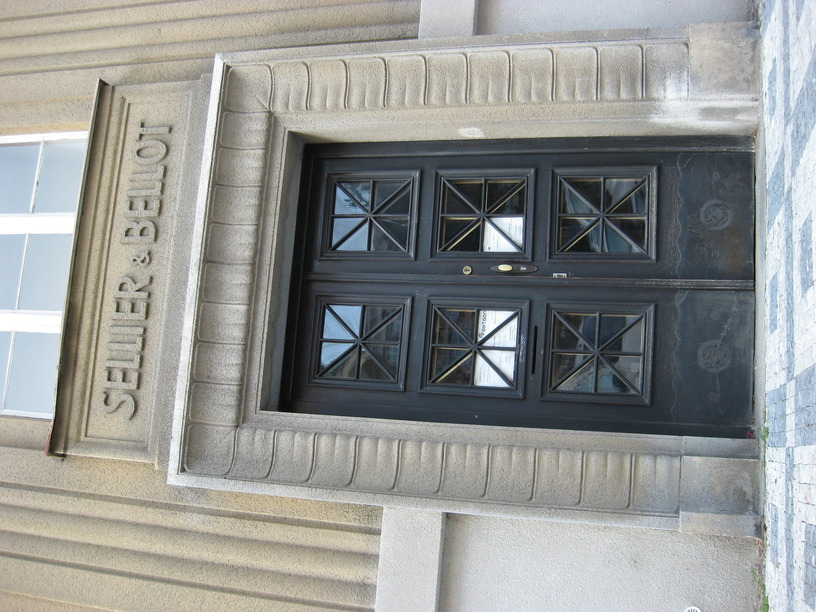
\includegraphics[width=4cm,angle=-90]{pictures/IMG_5953.JPG}}
			% }
			% \subfigure[] {
			% 	\fbox{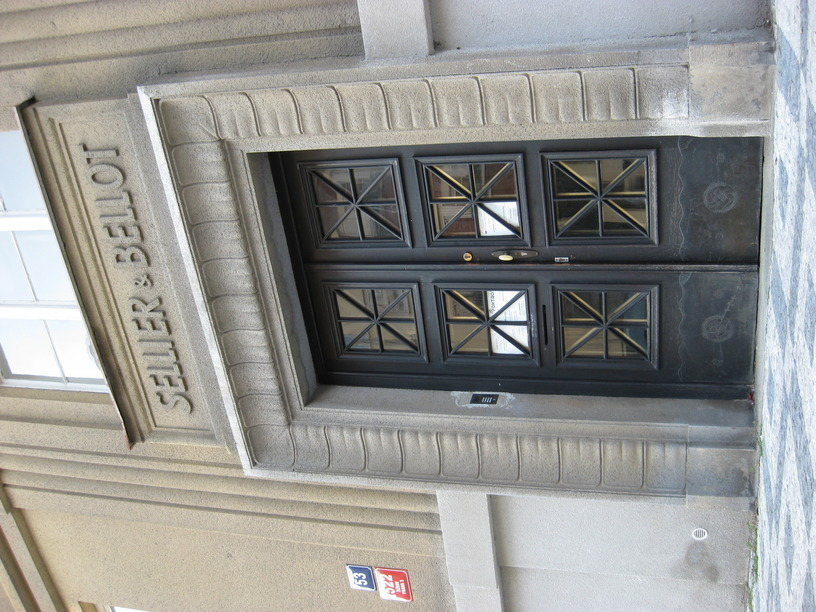
\includegraphics[width=4cm,angle=-90]{pictures/IMG_5960.JPG}}
			% }
			% \subfigure[] {
			% 	\fbox{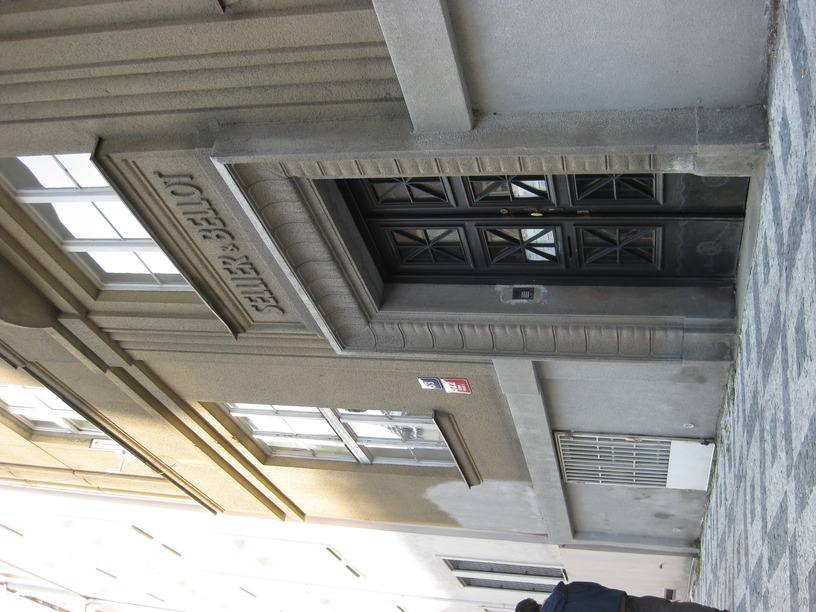
\includegraphics[width=4cm,angle=-90]{pictures/IMG_5963.JPG}}
			% }
		\caption{Snímky scény, které byly použity pro rekonstrukci, označení obrázků
			odpovídá označení kamer na obrázku \ref{fig:usporadaniKamer}}
		\label{fig:fotografie}
	\end{figure}

\paragraph{Odstranění radiálního zkreslení a kalibrace kamery} Protože použité algoritmy pra\-cují
s~lineárním modelem kamery, bylo nutné před dalším použitím nafocených snímků nejprve odstranit
radiální zkreslení. K tomuto účelu byl použit nástroj \emph{rd\_undistort}, který byl k dispozici od
vyučujících \cite{code_repo}.\footnote{Jak citovat tyto nástroje?} Jako podklad pro kalibraci tohoto
nástroje posloužily tři snímky vzoru zachyceného na obrázku~\ref{fig:radialCalibration}.
% \url{http://cmp.felk.cvut.cz/cmp/courses/TDV/code/rd\_undistort\_20110112.zip}

\def\IAC{\boldsymbol \omega}

K rekonstrukci scény je rovněž potřebná znalost vnitřní kalibrace použité kamery, tj. znalost
kalibrační matice $\matrix K$, která má obecně pět stupňů volnosti \cite[Determining Camera
Kalibration $\matrix K$ from a single view, str. 223]{Hartley2004}. U fotoaparátu jsme předpokládali
čtvercové pixely (bez zkosení), zbylé tři stupně volnosti kalibrační matice jsme určili na základě
úběžníků třech kolmých směrů v jediném obraze (viz. \figref{fig:kalibraceKamery}). Z každého páru
takových úběžníků $\vector u_i$, $\vector u_j$ vyplývá jedna podmínka na obraz absolutní
kuželosečky $\IAC$:
	\begin{equation}
		\vector u_i\T \IAC \vector u_j = 0, \qquad i, j \in \{1, 2, 3\},\quad i \ne j.
	\end{equation}
Kalibrační matici jsme určili z obrazu absolutní kuželosečky na základě vztahu
	\begin{equation} \IAC = (\matrix K \matrix K\T)^{-1} \end{equation}
pomocí Choleskyho faktorizace. Výsledná kalibrační matice byla:
	\begin{equation}
		\matrix K = \begin{pmatrix}
				3442,3	& 0		& 1614,3 \\
				0	& 3442,3	& 1185,7 \\
				0	& 0		& 1
			\end{pmatrix}.
	\end{equation}
	\begin{figure}[htb]
		\centering
		\subfigure[] {
			\fbox{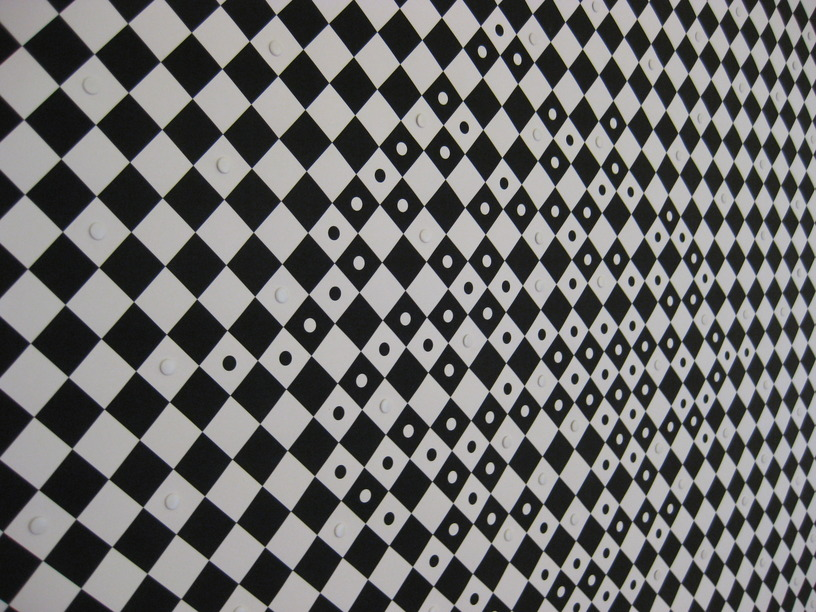
\includegraphics[width=7cm]{pictures/radial_calibration_pattern.jpg}}
			\label{fig:radialCalibration}
		}
		\subfigure[] {
			\fbox{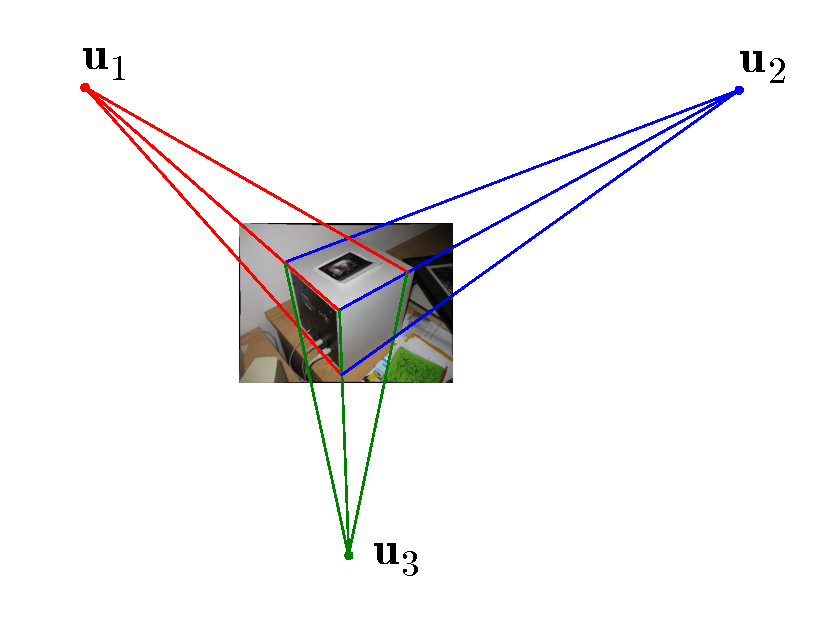
\includegraphics[width=7cm]{pictures/ubezniky_cube.pdf}}
			\label{fig:kalibraceKamery}
		}
		\caption{Snímky použité pro kalibraci: \subref{fig:radialCalibration} vzor použitý
			pro kalibraci nástroje pro odstranění radiálního zkreslení.
			\subref{fig:kalibraceKamery} Snímek kvádru použitého pro
			kalibraci kamery; červeně, zeleně a modře jsou vyznačeny rovnoběžky ve třech
			navzájem kolmých směrech protínající se v jednotlivých úběžnících.}
	\end{figure}

\paragraph{Nalezení řídkých korespondencí}

\paragraph{Odhad epipolární geometrie páru kamer}

- nalezení korespondencí -- opět byl použit nástroj dodaný učiteli - WBS matcher
- 5 bodový algoritmus \cite{stewenius-engels-nister-isprsj-2006}

% Notes:
%
% terminology:
%	correspondence = truth,
%	match = algorithm’s result; hypothesised corresp.


\section{Popis metody}

Pokusne citace:
\cite{SaraLectures}


	\begin{figure}[htb]
			\centering
			\subfigure[] {
				\fbox{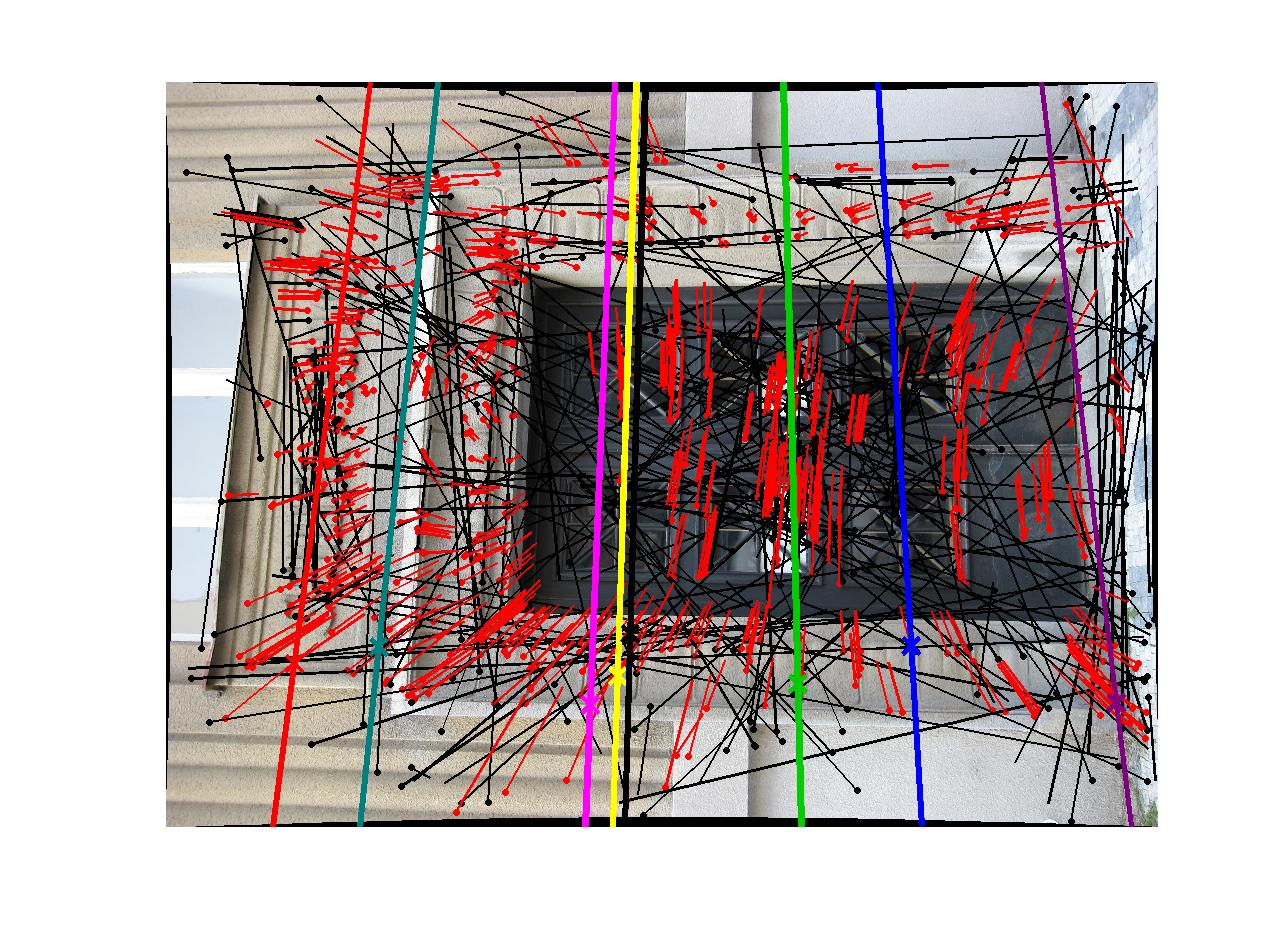
\includegraphics[width=8cm,angle=-90,clip=true,trim=165px 105px 110px 80px]{pictures/matches-left-with_epipolar_lines.jpg}}
			}
			\subfigure[] {
				\fbox{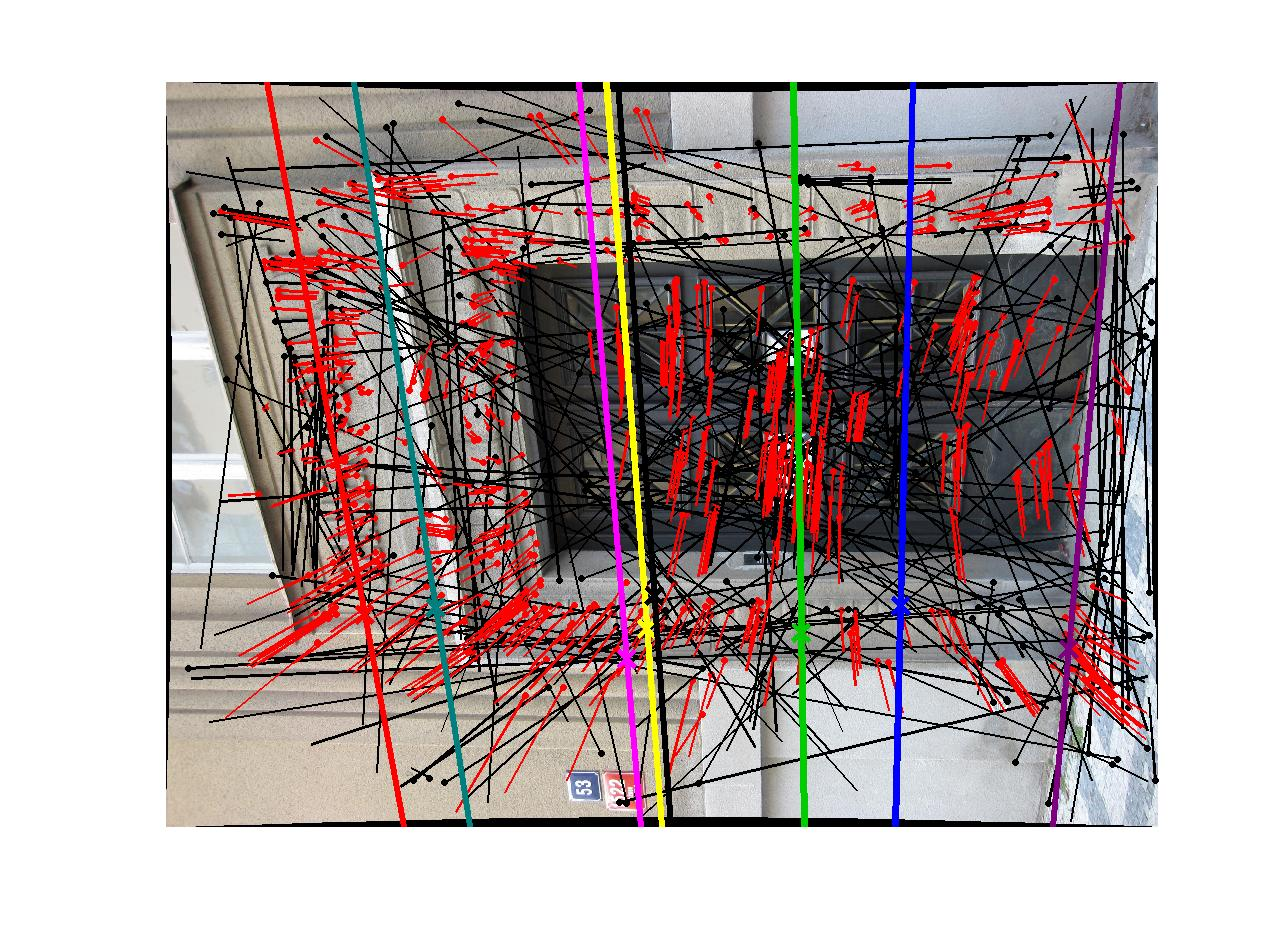
\includegraphics[width=8cm,angle=-90,clip=true,trim=165px 105px 110px 80px]{pictures/matches-right-with_epipolar_lines.jpg}}
			}
		\caption{Pár obrazů se zobrazenými korespondencemi: červeně korespondence odpovídající
			epipolární geometrii, černě chybné. Pro vybrané body (označené křížky) jsou
			stejnými barvami znázorněny vzájemně si odpovídající epipoláry. Obrazy
			odpovídají snímkům \ref{fig:i0} a \ref{fig:i1}. V obou obrazech je možné
			si všimnout podduškovitého obrysu okrajů, který vznikl po odstranění
			radiálního zkreslení.}
		\label{fig:pairWithEpipolars}
	\end{figure}

\section{Zhodnocení}

% FIXME: jak zahrnout bibliography.bib do repozitare? .. zkopirovat?

% Reference

	% FIXME:
	%	- zkontrolovat format oproti webu, zvolit vhodny .bst soubor
	%	- doplnit (?), aktualizovat odkazy a data

%\bibliographystyle{plain_cz}
\bibliographystyle{czechiso}
\bibliography{bibliography}

\end{document}

